\documentclass[11pt,letterpaper]{article}
\usepackage{samstyle}

\title{Daño en base de datos}
        
\author{
	Profesor\\
	Sergio Andres Monsalve Castañeda\\
	smonsal3@eafit.edu.co
}

\begin{document}
 
\pagestyle{fancyplain}
\fancyhf{}
\headheight=20pt %para cambiar el tamaño del encabezado
\renewcommand{\headrulewidth}{0pt} %espesor del encabezado

% \lhead %la "L" indica a la izquierda
% {
% }

\fancyfoot[c]{\thepage}

\maketitle

\begin{minipage}{3cm}
% 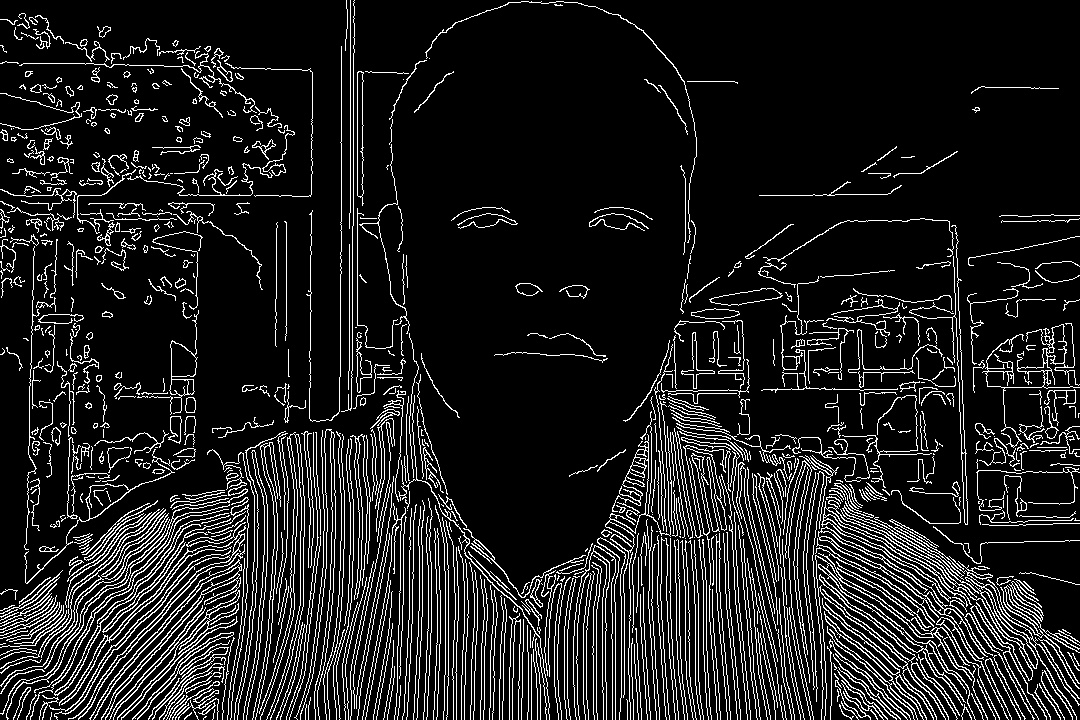
\includegraphics[width=15cm]{aux/SamCanny.jpg}
\end{minipage}


\section{Descripción}

En una base de datos de una universidad se daño una de las columnas de la tabla que contenia los estudiantes de un grupo. Pero se sabe que en tal tabla había solo 3 estudiantes y tenían el mismo nombre pero diferentes apellidos y codigos.

Se tienen los siguientes datos:

Apellido1 = ``Monsalve''
Apellido2 = ``Silva''
Apellido3 = ``Pineda''
Código1 = 200410061010
Código2 = 200120039010
Código3 = 199810043010


\section{Objetivo}

Nuestro objetivo es recuperar la integridad de la base de datos.

\section{Entrada}

Cuando la universidad nos diga cual fue el nombre que fue borrado nuestro programa deberá leer tal nombre como entrada, 

\section{Salida}

Se espera que su programa entregue como salida (Resultado) las siguientes lineas:

Nombre + espacio +  Apellido1 + espacio + codigo1 \\
Nombre + espacio +  Apellido2 + espacio + codigo2 \\
Nombre + espacio +  Apellido3 + espacio + codigo3 \\

\section{Ejemplo}
\subsection{Entrada}
\lstinputlisting{db.in}
\subsection{Salida}
\lstinputlisting{db.ot}

%\bibliographystyle{plainnat}
%\bibliography{refs}

\end{document}


